\section{Introduction}\label{sec:intro}

Suppose you drop a ball through a Galton board with $N$ rows of pegs. At the
first peg the ball goes left or right with probability $\frac12$ each. At every
later peg it repeats its previous direction with probability $p$ and switches
with probability $q=1-p$. This is the board of Problem 131 in Kagey's Open
Problem Collection~\cite{kagey131}, and one of his questions is when the middle
bin is exactly as likely as each of the two end bins. If $p$ is close to 1 the
ball rarely switches, so the ends win. If $p=\frac12$ the ball does a simple
random walk, so the middle wins. Paper~A~\cite{paperA} finds the crossing in
between. The middle catches up with the ends when the expected number of
switches $T=Nq$ is about $\log N$.

\begin{figure}[t]
\centering
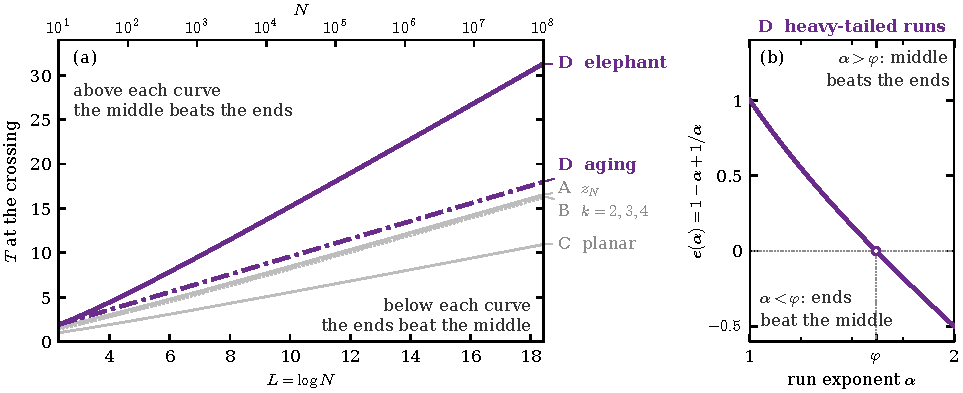
\includegraphics[width=0.8\textwidth]{../figures/program_D}
\caption{The crossing on each model's switching scale against $L=\log N$
(a), and the heavy-tailed exponent $e(\alpha)=1-\alpha+1/\alpha$ of this
paper for a stationary start (b). The scale is $T$ for Papers~A to~C,
$x=N\varepsilon$ for the elephant walk (drawn through the root $g_N$ of
Theorem~\ref{thm:erw-crossing}), and the expected number $H_N-1$ of
switches at the fixed-start crossing $c=1$ for the aging walk. The curves of
this paper are in bold, and a version of this figure also appears in
Paper~C.}
\label{fig:program}
\end{figure}

Kagey's ball remembers one step, since its next direction depends only on its
last one. In this paper we ask what happens to the middle-versus-ends question
if the ball remembers more. We study three kinds of memory.
\begin{itemize}[nosep]
\item In the elephant random walk of Sch\"utz and Trimper~\cite{schutz2004}
the ball remembers its whole past. At each peg it picks one of its earlier
directions uniformly at random and repeats it, except that with probability
$\varepsilon$ it reverses it. We write $x=N\varepsilon$, which is the expected
number of reversals up to $\varepsilon$.
\item In a walk with heavy-tailed runs the ball remembers how long it has
gone in its current direction. Its path is a sequence of runs of alternating
direction, and the run lengths $\xi$ are independent with
$\Prob(\xi\ge k)=k^{-\alpha}$ for $k\ge1$.
\item In an aging walk the ball remembers how old it is. It switches at peg
$k\ge2$ with probability $c/k$. We also give the ball $d$ directions. Then at
peg $k\ge2$ it turns to each of the other $d-1$ directions with probability
$\theta/(k+d-2)$, which is $c/k$ with $c=\theta$ when $d=2$.
\end{itemize}
The answer depends on the kind of memory. For the elephant walk the middle
needs about twice as many reversals as Kagey's board needs switches. Namely,
the crossing value of $x$ is about $2\log N$, not $\log N$. For heavy-tailed runs
started in equilibrium the ends win for large $N$ if $\alpha$ is below the
golden ratio $\varphi=(1+\sqrt5)/2$, and the middle wins if $\alpha$ is above
$\varphi$. For the aging walk with a fixed first step the crossing is exactly
$c=1$, for every $N$ and every bin. With $d$ directions the same happens at
$\theta=1$, where the vector of counts is exactly uniform
(Section~\ref{sec:aging}).

\paragraph{Why the elephant needs twice as many reversals.}
The ends are easy. The ball lands in the right end bin exactly when its first
step goes right and it never changes direction. This has probability
$\frac12(1-\varepsilon)^{N-1}\approx\frac12e^{-x}$ for the elephant walk, and
the same with $q$ in place of $\varepsilon$ for Kagey's board. So only the
middle differs. On Kagey's board the $T$ switches are spread over the whole
walk, and each moves the final position by about a run length $N/T$. So the
number of right steps spreads over about $N/\sqrt T$ bins, the middle bin has
probability of order $\sqrt T/N$, and the ends lose when $e^{-T}$ falls to
about $1/N$, that is, when $T\approx\log N$.

The elephant walk spreads a reversal in a different way. A reversal at step
$t+1$ is copied by later steps, those copies are copied, and so on. The steps
that descend from it form a family, whose share of the walk behaves like the
share of one ball in P\'olya's urn started with one ball against $t$. So a late
reversal has a small family and hardly moves the ball.
To land exactly in the middle, the walk needs a family that fills half the
walk, so it needs a reversal among its first few steps. This has probability
of order $\varepsilon$, and hitting the exact middle brings another factor of
order $1/N$. So the middle bin has probability of order $\varepsilon/N=x/N^2$ (in
fact about $4x/N^2$), and the ends lose only when $e^{-x}$ falls to about
$1/N^2$, that is, when $x\approx2\log N$. More precisely, at Kagey's crossing
$\frac12e^{-T}\approx\sqrt{2T/\pi}/N$, and squaring this relation turns it
into the elephant relation $\frac12e^{-x}\approx4x/N^2$ with
$x\approx2T-\log(2\pi)$.

The small families also give the shape of the law. About $x/m^2$ reversals
have a family of $m$ steps, so the bin at distance $m$ from an end has
probability about $x/(2m^2)$ over a wide range of $m$. So the law has a hump
near each end, and the middle is where the two tails meet. Indeed, twice
$x/(2m^2)$ at $m=N/2$ is the $4x/N^2$ above.

\paragraph{Why the golden ratio.}
For heavy-tailed runs take $1<\alpha<2$, so a run has a finite mean $\mu$ but
an infinite variance. Start the walk in equilibrium, at a typical time of a
long sequence of runs. Then the first run is already in progress, and long runs
are more likely to be in progress. The chance that this run covers all $N$
steps is of order $N^{1-\alpha}$, and this is the end. For the middle, the runs
to the right and the runs to the left form two independent renewal processes,
each making about $N/(2\mu)$ runs, and the ball ends in the middle when they
meet at level $N/2$. Each process fluctuates on the scale $N^{1/\alpha}$ of a
stable law, so they meet exactly with probability of order $N^{-1/\alpha}$. Hence the ratio of end to middle is
of order $N^{1-\alpha}/N^{-1/\alpha}=N^{1-\alpha+1/\alpha}$. The exponent
vanishes when $\alpha^2-\alpha-1=0$, that is, at $\alpha=\varphi$. Below
$\varphi$ the ends win, and above $\varphi$ the middle wins. If the first run
is a fresh run instead, the end is of order $N^{-\alpha}$, a factor $N$
smaller, and the middle wins for every $1<\alpha<2$.

\subsection{Relation to Papers A, B and C}\label{sec:series}

This is the fourth of four papers on Problem 131, which we call Papers~A, B, C
and~D. Paper~A~\cite{paperA} solves Kagey's board. Paper~B~\cite{paperB}
treats $d$ directions, where the ball turns to each other direction with the
same probability. Paper~C~\cite{paperC} gives the general theory for slowly
switching chains. These three papers study Markov walks, whose next step
depends only on the current one, and their answer is that the middle (or a
face) ties with the vertices when $T$ is of order $\log N$. This paper,
Paper~D, keeps Kagey's question and changes the walk. It can be read on its
own. From the earlier papers we use only the crossing equation of Paper~A,
namely~\eqref{eq:markov-crossing} below, and we use it only to compare the
elephant crossing with the Markov crossing in Section~\ref{sec:erw}. The four
papers share the following notation.
\begin{itemize}[nosep]
\item Kagey's board has $N$ steps (Kagey's row $n$ has $N=n-1$). The first
step is left or right with probability $\frac12$, and each later step repeats
the previous one with probability $p$. We put $q=1-p$ and $u=q/p$ (the odds of
a switch).
\item $P_N(k)$ is the probability of $k$ right steps, that is, the probability
that the ball lands in bin $k$. The endpoints have $P_N(0)=P_N(N)=p^{N-1}/2$.
\item $L=\log N$, and $T=Nq$ is the expected number of switches (up to the
first step).
\item The crossing is the value of $p$ (or of $T$) at which a bin is exactly
as likely as an endpoint. For the middle bin it is $p_N$, and
$z_N=N(1-p_N)$.
\item Papers~B and~C have $d$ states. A face $F$ is a nonempty set of states,
and the vertices are the faces of size $1$. For a chain with transition matrix
$I+(T/N)Q$, $\lambda_F$ is the principal Dirichlet eigenvalue of $-Q$ on $F$,
and $K_F$ is a second-order constant.
\end{itemize}
For the elephant walk $x=N\varepsilon$ corresponds to $T$, and its crossing
$x_N$ corresponds to $z_N$. We compare the two crossings through the crossing
equation of Paper~A~\cite[Proposition~3.8]{paperA}, which says that for every
$N\ge2$
\begin{equation}\label{eq:markov-crossing}
 z_N+\tfrac12\log z_N=L+c_0+\frac1{8z_N}+O(L^{-2}),\qquad
 c_0=\tfrac12\log\tfrac\pi8,
\end{equation}
where the error term is at most $\frac1{4L^2}+\frac{L^2+L}N$ in absolute
value, and that $L/2\le z_N\le L$. As in Paper~B the start law matters. For
heavy-tailed runs it decides whether the threshold is $\varphi$ or $1$, and
for the aging walk it decides whether the crossing is exactly $c=1$.
Figure~\ref{fig:program} shows the crossings of all four papers.

\subsection{Setting and notation}\label{sec:notation}

Every walk in this paper takes $N$ steps $X_1,\dots,X_N\in\{+1,-1\}$, where
$+1$ means right. Let $A_N=\#\{i\le N:X_i=+1\}$ be the number of right steps,
and keep writing $P_N(k)=\Prob(A_N=k)$ for the probability that the ball lands
in bin $k$, now for whichever walk we study. Unless we say otherwise the first
step is fair, $\Prob(X_1=+1)=\frac12$, and the rules treat the two directions
alike, so $P_N(k)=P_N(N-k)$. We write $\Prob_+$ and $\E_+$ for probability and
expectation given $X_1=+1$. For even $N$ we put $h=N/2$ and call
$C_N=P_N(h)$ the center and $E_N=P_N(N)=P_N(0)$ the end. Whenever $C_N$
appears, $N$ is even. The crossing is the value of the parameter at which
$C_N=E_N$. All logarithms are natural, $L=\log N$,
$H_k=\sum_{j\le k}1/j$ is the $k$-th harmonic number, and $\gamma$ is Euler's
constant. Limits, $O(\cdot)$ and $o(\cdot)$ refer to $N\to\infty$, over even
$N$ when $C_N$ appears. The constants implied by $O(\cdot)$ are absolute
unless we name what they depend on.

The elephant walk (Definition~\ref{def:erw}) has the reversal probability
$\varepsilon\in(0,1)$ and $x=N\varepsilon$. Its crossing is $\varepsilon_N$,
and $x_N=N\varepsilon_N$. Heavy-tailed runs (Section~\ref{sec:heavy}) have
the exponent $\alpha$, the mean run length $\mu=\E\xi=\zeta(\alpha)$ for
$\alpha>1$, and the length $D$ of the first run. A fresh start has $D$
distributed as $\xi$, and the stationary start has
$\Prob(D=d)=\Prob(\xi\ge d)/\mu$. We put $R_N=E_N/C_N$, so the ends win
exactly when $R_N>1$. The aging walk (Section~\ref{sec:aging}) has the
constant $c\in(0,2)$, and its version with $d$ states has the constant
$\theta$ and the count vector $(n_1,\dots,n_d)$, where $n_i$ is the number of
steps in state $i$. The symbols that only one section uses are defined at the start
of that section. The letters $p$, $q$ and $u$ have their meaning for Kagey's
board only in this introduction, and later sections reuse them locally.

\subsection{Results}\label{sec:results}

\paragraph{The elephant walk.}
For every even $N\ge2$ the crossing $\varepsilon_N$ exists, is unique and is
below $\frac12$ (Proposition~\ref{prop:mlr}). The center has derivative
exactly $4/(N+2)$ at $\varepsilon=0$
(Proposition~\ref{prop:first-mutation}), and
$C_N=\frac{4\varepsilon}{N+2}(1+O(\varepsilon\log N))$ for even $N\ge64$ and
$\varepsilon(1+\log N)\le\frac1{100}$, with explicit constants
(Theorem~\ref{thm:erw-bounds}). Let $g_N$ be the root of
$g+\log g=2L-\log8$. Then $x_N=g_N+O(L^2/N)$, and so
$x_N=2L-\log L-\log16+O(\log L/L)$ (Theorem~\ref{thm:erw-crossing}). Compared
with Kagey's board, $x_N=2z_N-\log(2\pi)+c_*/L+O(\log L/L^2)$ with
$c_*=\frac12\log(2\pi)-\frac14$ (Theorem~\ref{thm:erw-markov}).

We also go one order further. In the same range of $\varepsilon$ the center
is $\frac{4\varepsilon}{N+2}N^{2\varepsilon}(1+O(\varepsilon))$, with
explicit constants (Proposition~\ref{prop:second-order}). This gives
$x_N=g_N-(2g_NL+g_N^2/2)/(N(1+1/g_N))+O(L/N)$, so the root $g_N$ is above the
crossing for large $N$ (Proposition~\ref{prop:refined}). At fixed $N$ the
center is a polynomial $c_1\varepsilon+c_2\varepsilon^2+\cdots$ in
$\varepsilon$, and $c_2/c_1-2L\to2\gamma-2-\log2$
(Proposition~\ref{prop:K2}).

The remaining results describe the whole law near the crossing. At the
crossing the end is below its neighbor for every even $N\ge8$
(Corollary~\ref{cor:dip} and Proposition~\ref{prop:dip-hyp}). For $N<1688$
this rests on a floating-point computation whose rounding error we bound
(Lemma~\ref{lem:rounding}). Let $M_N$ be the number of steps that disagree
with the first step. For $N\ge2$ and $\varepsilon\le\frac14$ the law of $M_N$
is within an explicit $\delta_B$ of a compound Poisson law, bin by bin, and
$\delta_B=O(x^2\log^2N/N)$ when $x^2\le N$ (Theorem~\ref{thm:cp}). If
$x\to\infty$ and $x^3\log^2N/N\to0$, then $(M_N-x\log x)/x$ converges in law
to the Landau law, with a bound for each bin (Theorem~\ref{thm:landau}). So at
the crossing every mode lies at distance
$x_N\log x_N+\lambda_0x_N+O(\sqrt{x_N\log x_N})$ from the nearer end, where
$\lambda_0\approx-0.2228$ is the mode of the Landau density
(Corollary~\ref{cor:mode-location}, and Corollary~\ref{cor:modes} gives the
weaker bound $O(x_N\log^2x_N)$). Farther from the ends, bin $N-m$ has
probability $\frac x{2m^2}(1+o(1))$ for $x\log^2(x+1)\ll m\ll N$, when
$x\ge1$ and $x\log^2N/N\to0$ (Theorem~\ref{thm:profile}). Finally, for large
even $N$ the center at the crossing is below every interior bin outside a
window of width of order $N^{1/2}\log N$ around it
(Theorem~\ref{thm:shape}).

\paragraph{Heavy-tailed runs.}
For $1<\alpha<2$ and every first run that is finite almost surely, $C_N$ is
asymptotic to an explicit constant times $N^{-1/\alpha}$
(Theorem~\ref{thm:center}). With the stationary start
$R_N\sim C(\alpha)N^{1-\alpha+1/\alpha}$, and $C(\varphi)=0.7761\ldots$, so at
$\alpha=\varphi$ the center still wins. With a fresh start $R_N\to0$
(Corollary~\ref{cor:golden}). For $\alpha\ge2$ the center is of order
$N^{-1/2}$, with an extra factor $(\log N)^{-1/2}$ at $\alpha=2$, and
$R_N\to0$ with either start (Theorem~\ref{thm:alpha2}). For $0<\alpha<1$ the
runs have infinite mean and only the fresh start makes sense. Then
$NC_N\to\frac2\pi\tan\frac{\pi\alpha}2$ and $R_N\to\infty$
(Theorem~\ref{thm:lamperti}). So with a fresh start the ends win for
$\alpha<1$ and the center wins for $\alpha>1$. We do not prove what happens
at $\alpha=1$ (Remark~\ref{rem:other}).

\paragraph{Aging.}
With a fixed first step and $c=1$ the number of right steps is exactly
uniform on $\{1,\dots,N\}$. The ratio of each interior bin to the end
increases strictly in $c$, so every interior bin ties with the end exactly at
$c=1$, for every $N\ge2$ (Proposition~\ref{prop:aging-two}). With $d$ states,
a start in state~$1$ and $\theta=1$, the count vector is exactly uniform over
all compositions $(n_1,\dots,n_d)$ of $N$ with $n_1\ge1$, and every other
such bin ties with the corner $(N,0,\dots,0)$ exactly at $\theta=1$, for
every $N\ge2$ (Theorem~\ref{thm:aging-d}). A small change of the aging rate
gives a chain that redraws or repeats its state, and its counts have exactly
the law of P\'olya's urn for every weight
(Proposition~\ref{prop:aging-urn}). With a fair first step each
interior bin is twice as likely as an end at $c=1$, and its crossing is
unique and below $1$ (Proposition~\ref{prop:aging-fair}). For the center the
crossing is
$c_N=1-\log2/(\log N+\gamma+2-2\log2)+O((\log N)^{-3})$
(Proposition~\ref{prop:aging-expansion}).

\subsection{Prior work}\label{sec:prior}

The steps of the elephant walk split into clusters, since a step either
copies an earlier step exactly, with probability $1-2\varepsilon$, or starts
a new cluster with a fair sign. This is K\"ursten's coupling with bond
percolation on random recursive trees~\cite{kursten2016}, and Baur and
Bertoin~\cite{baurbertoin2016} relate the walk to P\'olya-type urns. Our
regime $N\varepsilon\asymp\log N$ lies in the strongly supercritical regime
of Baur~\cite{baur2016}, who extends the results of
Bertoin~\cite{bertoin2014} for retention probability $1-t/\log n$. Baur's
Corollary~1 gives the sizes of the largest clusters other than the root's (a
Poisson limit with intensity $a^{-2}\,da$), which is the picture of about
$x/m^2$ families of size $m$ behind Theorem~\ref{thm:profile}. These results
describe cluster sizes, not the center probability, which is a large deviation
of the root cluster. The law that appears in the bulk
(Theorems~\ref{thm:cp} and~\ref{thm:landau}) is also known. Without its
truncation, our compound Poisson law is the Lea--Coulson form of the
Luria--Delbr\"uck distribution, and Kessler and
Levine~\cite[Eqs.~(14), (18) and~(19)]{kesslerlevine2015} describe its profile
$x/(m(m+1))$ for small $x$ and its Landau limit for large $x$ (see
also~\cite{mohle2005}). The same stable law governs the fluctuations of the
root cluster when the retention probability is
$1-c/\log n$~\cite{bertoin2014ejp}. What we add is the comparison of the
elephant walk with this law in our regime (with an explicit error in
Theorem~\ref{thm:cp}) and a certified enclosure of the mode.
Gu\'erin, Laulin, Raschel and Simon~\cite[proof of Theorem~1.1]{glrs2025}
prove that the law with a fixed first step is unimodal, and their other
results fix the memory parameter as $N$ grows. So do the local limit theorem
of Trinas and Valle~\cite[Theorem~3.1]{tv2026} for the superdiffusive walk
and their bounds on where log-concavity fails. We did not find an asymptotic
formula for the center probability when $\varepsilon\to0$ as $N$ grows.

For heavy-tailed runs, Godr\`eche and Luck~\cite{godrecheluck2001} give the
transform of the occupation time of an alternating renewal process and the
scalings of the center and of both edges, and~\cite{zdk2015,dsd2013} describe
the profile of a L\'evy walk. Wang, Li and H\"anggi~\cite{wlh2016} already observe,
as a heuristic for heat conduction, that equal decay of the central peak and
the side peaks gives the golden ratio. The two decay rates of the end,
$N^{1-\alpha}$ and $N^{-\alpha}$, are the scalings of the ballistic peaks of a
L\'evy walk with and without an equilibrated start~\cite[Table~I]{dzh2012}. We
prove the lattice statement with a local limit at the center, treat both
starts, and compute $C(\alpha)$. For $\alpha<1$ the limit law of $A_N/N$ is
Lamperti's~\cite{lamperti1958}.
For aging walks, Dietz and Sethuraman~\cite{ds2007} proved the limit law of
$A_N/N$, Engl\"ander and Volkov~\cite{ev2018} gave a second proof, and
Engl\"ander, Volkov and Wang~\cite{evw2020} found the scaling limit of the
walk. For $d$ states the limit is a Dirichlet
law~\cite[Theorem~1.4]{ds2007}. The exact uniform law for two states is an
exercise in~\cite[footnote~1 on p.~6]{evw2020}, which also announces a general
connection with P\'olya urns, and the chain that redraws or repeats is a
conservative random walk in the sense of~\cite{ev2022}. What is new in
Section~\ref{sec:aging} is the explicit joint law of the counts and the last
state for $d$ states and the ties that follow from it.

\subsection{Organization}\label{sec:organization}

Section~\ref{sec:erw} reduces the elephant walk to a counting chain, proves
that its crossing is unique, finds the crossing, and then gives the center
and the crossing to second order. Section~\ref{sec:shape} describes the whole
law near the crossing, namely the dip at each end, the compound Poisson and
Landau approximations of the bulk with the place of the modes, the tail
$x/(2m^2)$, and the window around the center. Section~\ref{sec:heavy} treats
heavy-tailed runs, first the golden ratio for $1<\alpha<2$ and then the
exponents $\alpha\ge2$ and $\alpha<1$. Section~\ref{sec:aging} treats the
aging walk with a fixed first step, with $d$ states, and with a fair first
step. Section~\ref{sec:verify} describes the checks. The longer proofs are in
the appendices. Appendix~\ref{app:erw} holds the proofs for
Section~\ref{sec:erw}. Appendix~\ref{app:shape} holds the proofs for the
tail and the modes in Section~\ref{sec:shape}, and Appendix~\ref{app:bulk}
holds the proofs for the bulk. Appendix~\ref{app:heavy} holds the proofs for
Section~\ref{sec:heavy}, and Appendix~\ref{app:aging} proves
Proposition~\ref{prop:aging-expansion}.
